\newpage 
\null 
\vspace{0.15cm}

\begin{center} 
\Huge{\textbf{\underline{Chapter 6: PL/SQL}}}

\end{center}

\setcounter{section}{0}

\vspace{0.35cm}

\section{Introduction}

\begin{prettyBox}{What's PL/SQL ?}{myblue}
PL/SQL, or Procedural Language/Structured Query Language, is an extension of SQL. While SQL (Structured Query Language) is primarily used for CRUD operations (querying, inserting, updating, and deleting data in relational databases), PL/SQL allows for full programmatic control with features such as control structures (loops and conditionals), variables, and error handling with exceptions. This enables the creation of scripts that can automate tasks with functions, procedures, and triggers, implement complex business logic, and manipulate data at a higher level than SQL alone.
\end{prettyBox}

\vspace{0.25cm}

\begin{prettyBox}{Differences Between PL/SQL and SQL}{myblue}
\begin{itemize}
    \item SQL is limited to CRUD operations; PL/SQL adds procedural programming capabilities.
    \item PL/SQL provides advanced error handling through exceptions.
    \item PL/SQL supports modular programming with functions, procedures, and triggers.
    \item PL/SQL is specific to Oracle databases, whereas SQL is standardized across various databases.
\end{itemize} 
\end{prettyBox}

\vspace{0.5cm}

\section{Overview Of Plsql's Structure}

\begin{prettyBox}{Programme Structure}{myblue}
A PL/SQL has 3 blocks :
\begin{itemize}
    \item \textbf{DECLARE}(Optional Block) : contains all the declared variables , constants \& modules(functions,procedure) 
    \item \textbf{MAIN} : contains the main executable code 
    \item \textbf{EXCEPTION}(Optional Block) : handls erros with exceptions 
\end{itemize}
\end{prettyBox}

\begin{center}
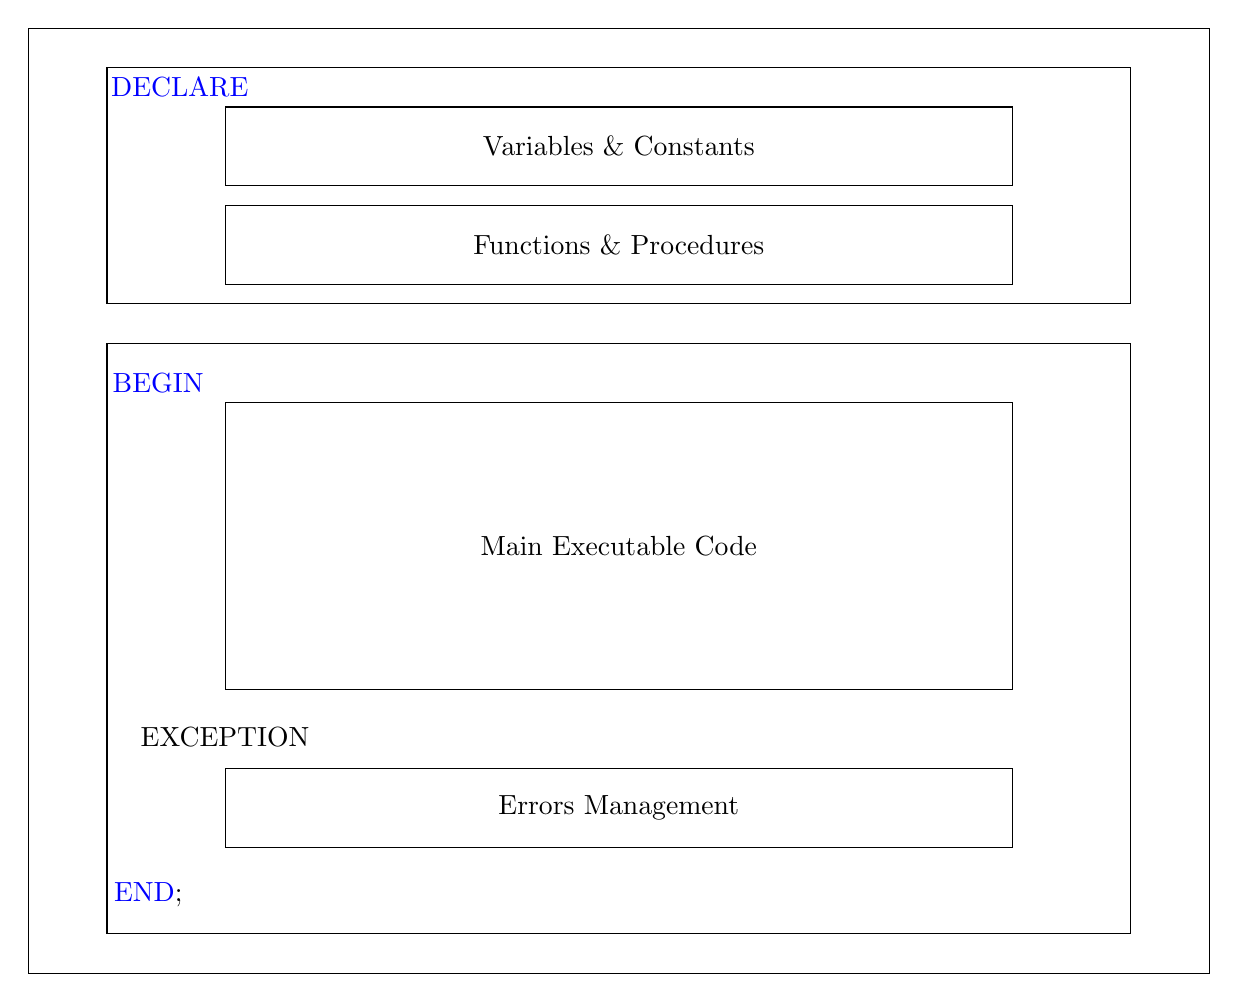
\begin{tikzpicture}
    \draw (0,0) rectangle (15,12);
    
    \draw (1,8.5) rectangle(14,11.5);
    \node at (1.925,11.25) {\textcolor{blue}{DECLARE}};
    \draw (2.5,10) rectangle (12.5,11);
    \node at(7.5,10.5){Variables \& Constants};
    \draw (2.5,8.75) rectangle (12.5,9.75);
    \node at (7.5,9.25){Functions \& Procedures};
    
    \draw (1,0.5) rectangle(14,8);
    \node at (1.65,7.5) {\textcolor{blue}{BEGIN}};
    \draw (2.5,3.6) rectangle (12.5,7.25);
    \node at (7.5,5.425){Main Executable Code};
    \node at (2.5,3) {EXCEPTION};
    \draw (2.5,1.6) rectangle (12.5,2.6);
    \node at (7.5,2.1){Errors Management};
    \node at (1.525,1) {\textcolor{blue}{END};};
\end{tikzpicture}
\end{center}

\vspace{0.5cm}

\section{Comments}


\subsection*{\underline{Syntax}}

\vspace{0.25cm}

\subsection*{\underline{Single Comment}}
\lstinputlisting{SQL/syntax/Pl_Sql/singleComment.sql}


\subsection*{\underline{Multi-Line Comment}}
\lstinputlisting{SQL/syntax/Pl_Sql/multiComment.sql}


\vspace{0.5cm}


\section{Printing}

\begin{prettyBox}{DBMS\_OUTPUT.PUT\_LINE}{myblue}
To print messages in the console, we use the \texttt{DBMS\_OUTPUT.PUT\_LINE} command. The message should be enclosed
in single quotes ' ' and we use double pipes \texttt{||} to concatenate with variables.
\end{prettyBox}

\subsection*{\underline{Syntax}}


\lstinputlisting{SQL/syntax/Pl_Sql/print.sql}

\vspace{0.25cm}

\begin{prettyBox}{Note}{red}
To be able to see the printed messages in the console of SQL*Plus, SQL Developer, ...etc, we need to activate
the buffer responsible for printing the messages by using the command: 

\lstinputlisting{SQL/syntax/Pl_Sql/server.sql}

Note that this is only needed once , and it will remain active unless you explicitly turn it off.
\end{prettyBox}

\vspace{0.5cm}

\section{Variables Declaration \& Types}

\begin{prettyBox}{Variables \& Constants}{myblue}
All variables and constants must be declared in the \textcolor{blue}{DECLARE} scope , 
we use := to affect values to variables 
\end{prettyBox}

\subsection*{\underline{Syntax}}

\lstinputlisting{SQL/syntax/Pl_Sql/varDeclaration.sql}

\vspace{0.25cm}
\begin{prettyBox}{Types}{myblue}
PL/SQL supports all data types normal sql has like those we've seen previously. Here, we introduce two additional types:

\begin{itemize}
    \item \textbf{Type:} Used to define a variable with the same data type as a column in a table:
    
\lstinputlisting{SQL/syntax/Pl_Sql/type.sql}

    \item \textbf{RowType:} Used to define a variable as a record with the structure of a row in a table:
\lstinputlisting{SQL/syntax/Pl_Sql/rowType.sql}
\end{itemize}

\end{prettyBox}



\begin{prettyBox}{Store Select Output In Variables}{myblue}
We can store the output of the \textcolor{blue}{SELECT} command in variables using the \textcolor{blue}{INTO} clause as follows:
\end{prettyBox}

\subsection*{\underline{Syntax}}

\lstinputlisting{SQL/syntax/Pl_Sql/select.sql}

\vspace{0.25cm}

\begin{prettyBox}{Note}{red}
\textbf{\underline{Order Of Variables Is Important}}

\vspace{0.15cm}
The order of the variables in the \textcolor{blue}{INTO} clause must match the order of the selected columns

\vspace{0.25cm}
\textbf{\underline{Select Should Ouput One Line Only}}

\vspace{0.15cm}
When Storing the output of \textcolor{blue}{SELECT} in variables , the ouput should be one line and not a table
if not we will have to use cursor to navigate through the table we will cover that later on


\vspace{0.25cm}

\textbf{\underline{We Must Use Store Select Output}}

\vspace{0.15cm}
In PL/SQL we have to always store the output of a select if not we will have a complilation error
\end{prettyBox}

\vspace{0.5cm}
\section{Control Structures}

\begin{prettyBox}{Definition}{myblue}
In PL/SQL, control structures are constructs that help control the flow of execution in a block of code.
They determine the order and conditions under which statements are executed and help make the code dynamic
and responsive to varying conditions. The main types of control structures in PL/SQL are:
\end{prettyBox}

\vspace{0.25cm}

\subsection{Conditional Control}
\newpage
\subsubsection{\underline{If}} 
\subsubsection{\underline{Syntax}}

\lstinputlisting{SQL/syntax/Pl_Sql/if.sql}


\vspace{0.25cm}

\subsubsection{\underline{Switch Case}}

\subsection*{\underline{Syntax}}

\lstinputlisting{SQL/syntax/Pl_Sql/case.sql}

\vspace{0.25cm}

\subsection{Looping Control}

\subsubsection{\underline{Simple Loop}}


\subsection*{\underline{Syntax}}


\lstinputlisting{SQL/syntax/Pl_Sql/simpleLoop.sql}



\subsubsection{\underline{While Loop}}

\subsection*{\underline{Syntax}}


\lstinputlisting{SQL/syntax/Pl_Sql/whileLoop.sql}


\vspace{0.25cm}



\subsubsection{\underline{For Loop}}

\subsection*{\underline{Syntax}}


\lstinputlisting{SQL/syntax/Pl_Sql/forLoop.sql}

\vspace{0.5cm}

\section{Raise Application Error}
\begin{prettyBox}{Raise Errors}{myblue}
RAISE\_APPLICATION\_ERROR is a procedure used to raise an error that halts code execution, with a custom error
message. Each error\_code (between -20000 and -20999) is associated with an error message retrieved 
by SQLERRM, while SQLCODE captures the error code itself.

\vspace{0.25cm}


\lstinputlisting{SQL/syntax/Pl_Sql/raise_application.sql}

\vspace{0.25cm}


Though commonly used to handle user-defined exceptions, RAISE\_APPLICATION\_ERROR can also be used internally
by the system for predefined exceptions, supporting error control in both system and custom PL/SQL operations.
\end{prettyBox}

\newpage
\subsection*{\underline{Syntax}}


\lstinputlisting{SQL/syntax/Pl_Sql/raise.sql}


\vspace{0.5cm}

\section{Exceptions}
\begin{prettyBox}{Exception}{myblue}
Exceptions help manage errors . Under
the hood, exceptions are built on RAISE\_APPLICATION\_ERROR ,  only difference is that it's more readable. There are two main types of exceptions:
\begin{itemize}
    \item \textbf{Predefined Exceptions}: These are system-defined exceptions, such as:
        \begin{itemize}
            \item NO\_DATA\_FOUND: Raised when a \textcolor{blue}{SELECT} statement returns no rows.
            \item TOO\_MANY\_ROWS: Raised when a \textcolor{blue}{SELECT} statement returns more than one row.
        \end{itemize}
    \item \textbf{User-defined Exceptions}: Defined by the user using the \textcolor{blue}{EXCEPTION} DataType.
\end{itemize}
\end{prettyBox}

\newpage
\subsection*{\underline{Syntax}}


\lstinputlisting{SQL/syntax/Pl_Sql/exc.sql}




\vspace{0.5cm}
\begin{prettyBox}{Note}{red}
\textbf{\underline{What is OTHERS?}}

\vspace{0.15cm}
It’s best practice to add OTHERS as the last exception handler, as it catches any exceptions not explicitly
defined. This ensures any unexpected errors are managed gracefully.

\vspace{0.25cm}

\textbf{\underline{When to Use RAISE\_APPLICATION\_ERROR vs. Exceptions?}}

\vspace{0.15cm}
Although exceptions are built on RAISE\_APPLICATION\_ERROR, they offer better readability and manageability
in complex code. Use exceptions for organized error handling, while RAISE\_APPLICATION\_ERROR provides a more
direct and minimalistic approach.
\end{prettyBox}

\newpage

\section{Cursor}
\begin{prettyBox}{Cursor}{myblue}
Cursors are used when a \textcolor{blue}{SELECT} query returns a table (more than one row).  
To use a cursor, we first declare a variable of the \textcolor{blue}{CURSOR} data type and associate it with a \textcolor{blue}{SELECT} query.\\[0.15cm]
Then, inside the BEGIN-END block, we perform the following steps:  

\begin{itemize}
    \item Open the cursor using the \textcolor{blue}{OPEN} keyword.  
    \item Load the first row using the \textcolor{blue}{FETCH} keyword and store the output in variables.  
    \item Loop through the table using the \textcolor{blue}{FOUND} function, which is a boolean function that returns \textbf{true} if a row is successfully loaded.  
\end{itemize}

Inside the WHILE loop: 
\begin{itemize}
    \item Process the current row.  
    \item Load the next row using \textcolor{blue}{FETCH}.  
\end{itemize}

When \textcolor{blue}{FOUND} returns false, indicating no more rows, the loop exits. Finally, close the cursor using the \textcolor{blue}{CLOSE} keyword to free up memory.  
\end{prettyBox}

\subsection*{\underline{Syntax}}

\lstinputlisting{SQL/syntax/Pl_Sql/cursor.sql}


\section{Trigger}

\begin{prettyBox}{Trigger}{myblue}
Triggers are standalone PL/SQL code blocks that execute automatically in response to a specified event.  

\vspace{0.15cm}
There are two types of triggers:  
\begin{itemize}
    \item Row-level triggers  
    \item Table-level triggers  
\end{itemize}

Triggers can be associated with various events, such as \textcolor{blue}{INSERT}, \textcolor{blue}{UPDATE}, or \textcolor{blue}{DELETE}.  

\vspace{0.15cm}
They are useful for automating tasks, enforcing rules, or logging changes.  
\end{prettyBox}

\subsection*{\underline{Syntax}}

\lstinputlisting{SQL/syntax/Pl_Sql/trigger.sql}



\subsection{Row Level Trigger}

\begin{prettyBox}{Row Level}{myblue}
We use the \textcolor{blue}{FOR EACH ROW} keyword, which instructs the trigger
to execute for every row that is deleted or updated.

This also provides us with access to:
\begin{itemize}
    \item :\textcolor{blue}{NEW}.colName – This gives the value of a column for the newly inserted or updated row.
    \item :\textcolor{blue}{OLD}.colName – This gives the value of a column for a deleted row or the value before an update.
\end{itemize}

We use row-level triggers when we need to access :\textcolor{blue}{NEW} and :\textcolor{blue}{OLD}, or when the event is row-specific, such as \textcolor{blue}{DELETE} or \textcolor{blue}{UPDATE}.
\end{prettyBox}\newpage

\subsection*{\underline{Syntax}}

\lstinputlisting{SQL/syntax/Pl_Sql/rowLevel.sql}




\subsection{Table Level Trigger}

\begin{prettyBox}{Table Level}{myblue}
A trigger is considered table-level if we omit the \textcolor{blue}{FOR EACH ROW} keyword. Unlike row-level triggers, table-level triggers do not have access to \textcolor{blue}{:NEW} and \textcolor{blue}{:OLD}.

\vspace{0.15cm}
We use table-level triggers when:
\begin{itemize}
    \item There is no need to access \textcolor{blue}{:NEW} or \textcolor{blue}{:OLD} values.
    \item The event is not row-specific, such as when performing actions like \textcolor{blue}{DROP}, \textcolor{blue}{ALTER}, or other table-wide operations.
    \item We want to override a command using \textcolor{blue}{INSTEAD OF}.
\end{itemize}
\end{prettyBox}

\subsection*{\underline{Syntax}}

\lstinputlisting{SQL/syntax/Pl_Sql/tableLevel.sql}




\subsection{Trigger Events}

\begin{prettyBox}{Events}{myblue}
Triggers are defined for different types of events, which can be categorized as follows:

\vspace{0.2cm}
\textbf{\underline{Trigger Types}:}
\begin{itemize}
    \item \textcolor{blue}{BEFORE} : The trigger executes before an event.
    \item \textcolor{blue}{AFTER} : The trigger executes after an event.
    \item \textcolor{blue}{INSTEAD OF} : The trigger overrides the event entirely (typically used with views).
\end{itemize}

\textbf{\underline{Operations}:}
\begin{itemize}
    \item \textcolor{blue}{INSERT} on tableName : Trigger fires when a row is inserted into the table.
    \item \textcolor{blue}{DELETE} on tableName : Trigger fires when a row is deleted from the table.
    \item \textcolor{blue}{UPDATE} on tableName : Trigger fires when a row is updated in the table.
    \item \textcolor{blue}{UPDATE} of columnName on tableName : Trigger fires when a specific column in the table is updated.
    \item \textcolor{blue}{DROP} on tableName : Trigger fires when a table is dropped .
\end{itemize}

You can use the \textcolor{blue}{OR} keyword in a trigger definition to specify multiple events for the same table. This allows the trigger to fire on different types of events.
\end{prettyBox}

\subsection*{\underline{Syntax}}

\lstinputlisting{SQL/syntax/Pl_Sql/event.sql}




\begin{prettyBox}{Note}{red}
\textbf{\underline{A Trigger Can Be Linked to Only One Table}}

\vspace{0.15cm}
A trigger can only be linked to a single table. Therefore, attempting something like 
BEFORE \textcolor{blue}{UPDATE} ON table1 \textcolor{blue}{OR} AFTER \textcolor{blue}{INSERT} ON table2 is incorrect.

\vspace{0.25cm}

\textbf{\underline{Avoid Using Multiple Events in a Single Trigger}}

\vspace{0.15cm}
It is generally not considered a best practice to combine multiple events with the \textcolor{blue}{OR} keyword in a single trigger. This can make the trigger logic harder to maintain and understand.\\[0.15cm]
\textbf{\underline{Mutated Table}}\\[0.15cm]
If we have a trigger that executes after insert/delete/update on a table, trying to read or modify that same table will result in mutated table error because trigger is trying to read or modify a table while it is inserting,deleting,updating\\[0.25cm]
\textbf{\underline{update on column}}\\[0.15cm]
We can create trigger that executes when only a certain column is being updated by using of
\begin{lstlisting}
after/before of columnName on tableName
\end{lstlisting}
\end{prettyBox}

\newpage
\section{Function}


\subsection*{\underline{Syntax}}

\subsection*{\underline{Function Definition}}

\subsection*{\underline{Local Function}}


\lstinputlisting{SQL/syntax/Pl_Sql/funcLocal.sql}

\newpage

\subsection*{\underline{Stand Alone Function}}

\lstinputlisting{SQL/syntax/Pl_Sql/funcAlone.sql}

\subsection*{\underline{Function Call}}

\subsection*{\underline{Inside Begin End Block}}

\lstinputlisting{SQL/syntax/Pl_Sql/funcCall.sql}

\subsection*{\underline{Call Directly With Exec}}

\lstinputlisting{SQL/syntax/Pl_Sql/exec.sql}

\vspace{0.25cm}

\begin{prettyBox}{Note}{red}
\textbf{\underline{Standalone vs. Local Functions and Procedures}}
\begin{itemize}
    \item \textbf{Standalone:} These are stored in the DBMS schema and can be called from anywhere.
    \item \textbf{Local:} These are defined inside the `DECLARE` block and can only be accessed or called within the same PL/SQL code.
\end{itemize}

\vspace{0.25cm}

\textbf{\underline{Common Errors in Parameters}}

\begin{itemize}
    \item You cannot use `TYPE` or `ROWTYPE` in parameter definitions.
    \item You cannot specify a size for `CHAR` or `VARCHAR2` in parameters.
\end{itemize}
\end{prettyBox}



\vspace{0.5cm}
\section{Procedure}

\subsection*{\underline{Syntax}}

\subsection*{\underline{Procedure Definition}}

\subsection*{\underline{Local Procedure}}


\lstinputlisting{SQL/syntax/Pl_Sql/proLocal.sql}


\subsection*{\underline{Stand Alone Procedure}}

\lstinputlisting{SQL/syntax/Pl_Sql/proAlone.sql}

\newpage
\subsection*{\underline{Procedure Call}}

\subsection*{\underline{Inside Begin End Block}}

\lstinputlisting{SQL/syntax/Pl_Sql/proCall.sql}

\subsection*{\underline{Call Directly With Exec}}

\lstinputlisting{SQL/syntax/Pl_Sql/proExec.sql}

\vspace{0.35cm}

\subsection*{\underline{Example}}
let the table definition be :\\[0.2cm]
\textbf{Client}(\textbf{\underline{numClient}},CIV,firstName,lastName,DOB,address,telProf,telPriv,fax);\\[0.1cm]
\textbf{Employee}(\textbf{\underline{numEmployee}},firstName,lastName,category,salary)\\[0.1cm]
\textbf{Brand}(\textbf{\underline{numBrand}},name,country)\\[0.1cm]
\textbf{Model}(\textbf{\underline{numModel}},numBrand*,name)\\[0.1cm]
\textbf{Vehicule}(\textbf{\underline{numVehicule}},numClient*,numModel*,mat,year)\\[0.1cm]
\textbf{Interventions}(\textbf{\underline{numIntervention}},numVehicule*,type,datebegin,dateend,cost)\\[0.1cm]
\textbf{Intervenants}(\textbf{\underline{numIntervention*,numEmployee}},datebegin,dateend)


\begin{enumerate}
    \item create the tables
    \item add constraint on salary so it's between 10000 and 30000 
    \item create a procedure that print how much each brand has models
    \item create a procedure that add 30\% in salary of employee with category 'Assistant' and 50\% for 'Mechanician'
    \item create a procedure that verifies wether the datebegin is inferior to dateend in the interventions table
    \item create a function that return for a given numemployee number of interventions
    \item create a trigger that notify when ever a new model is added to the brand
    \item create a trigger that verifies if the newly updated salary is greater than the older one if not , don't let it happen
    \item create a trigger that checks if the intervenants time respect the period of the intervention if not don't allow the insertion
    \item add the attribut nb\_inter total number of intervention of an employee
    \item create procedure that fills nb\_inter
    \item create trigger to automatically increment/decrement nb\_inter
\end{enumerate}

\newpage

\vspace{0.35cm}
\subsection*{\underline{1 Table Creation}}
\subsection*{1.1 Client Table}
\lstinputlisting{SQL/examples/PLSQL/EX1/ex1.1.sql}

\subsection*{1.2 Employee Table}
\lstinputlisting{SQL/examples/PLSQL/EX1/ex1.2.sql}

\subsection*{1.3 Brand Table}
\lstinputlisting{SQL/examples/PLSQL/EX1/ex1.3.sql}

\subsection*{1.4 Model Table}

\lstinputlisting{SQL/examples/PLSQL/EX1/ex1.4.sql}

\newpage
\subsection*{1.5 Vehicule Table}
\lstinputlisting{SQL/examples/PLSQL/EX1/ex1.5.sql}

\subsection*{1.6 Interventions Table}
\lstinputlisting{SQL/examples/PLSQL/EX1/ex1.6.sql}

\subsection*{1.7 Intervenants Table}

\lstinputlisting{SQL/examples/PLSQL/EX1/ex1.7.sql}

\newpage
\subsection*{2 Print Number Of Modals For Each Brand}

\lstinputlisting{SQL/examples/PLSQL/EX1/ex2.sql}

\vspace{0.25cm}
\begin{figure}[ht]
    \centering
    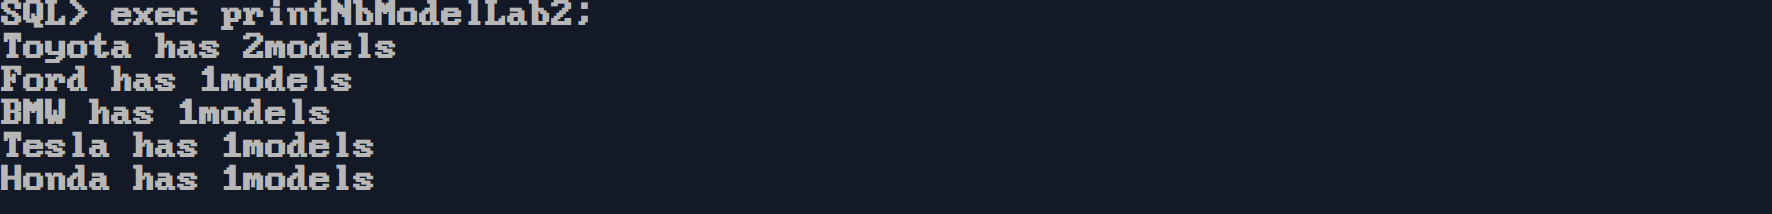
\includegraphics[width=\textwidth]{SQL/examples/PLSQL/EX1/PNG/ex2.png}
\end{figure}

\vspace{0.5cm}
\subsection*{3 Salary Constraint}

\lstinputlisting{SQL/examples/PLSQL/EX1/ex3.sql}

\newpage
\subsection*{4}

\subsection*{4.1 Disable Salary Constraint}

\lstinputlisting{SQL/examples/PLSQL/EX1/ex4.1.sql}

\subsection*{4.2 Procedure To Update Salary}

\lstinputlisting{SQL/examples/PLSQL/EX1/ex4.2.sql}

\newpage
\begin{figure}[ht]
    \centering
    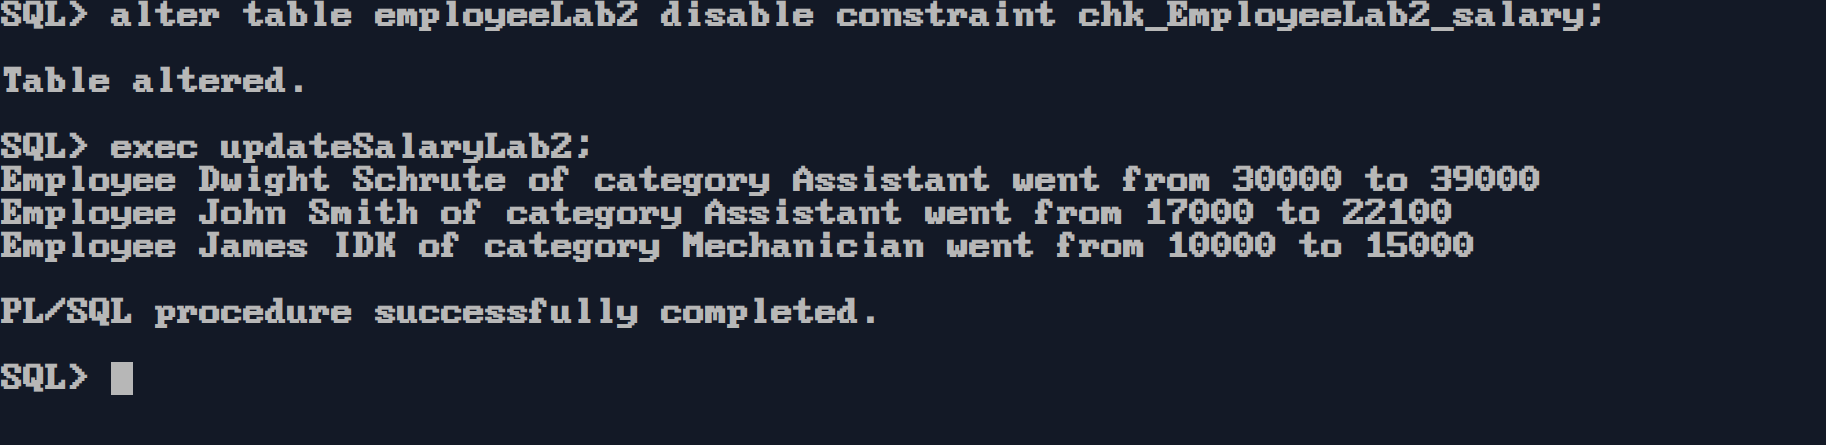
\includegraphics[width=\textwidth]{SQL/examples/PLSQL/EX1/PNG/ex4.png}
\end{figure}

\vspace{0.5cm}

\subsection*{5}

\subsection*{5.1 Verification For One Intervention}

\lstinputlisting{SQL/examples/PLSQL/EX1/ex5.1.sql}

\newpage
\subsection*{5.2 Verification For All Intervention}

\lstinputlisting{SQL/examples/PLSQL/EX1/ex5.2.sql}

\vspace{0.25cm}
\begin{figure}[ht]
    \centering
    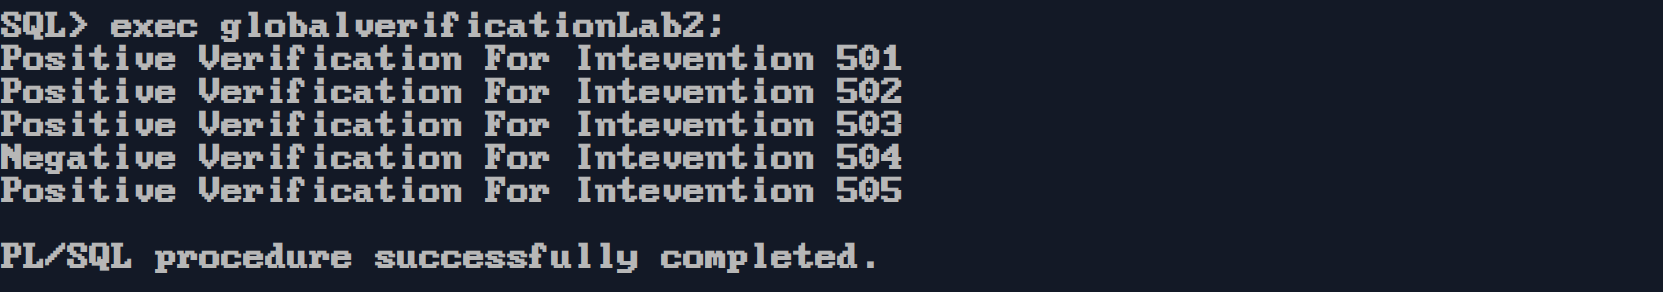
\includegraphics[width=\textwidth]{SQL/examples/PLSQL/EX1/PNG/ex5.png}
\end{figure}

\newpage

\subsection*{6}

\subsection*{6.1 Nb Interventions For One Employee}

\lstinputlisting{SQL/examples/PLSQL/EX1/ex6.1.sql}


\subsection*{6.2 Nb Interventions For All Employees}

\lstinputlisting{SQL/examples/PLSQL/EX1/ex6.2.sql}

\newpage
\begin{figure}[ht]
    \centering
    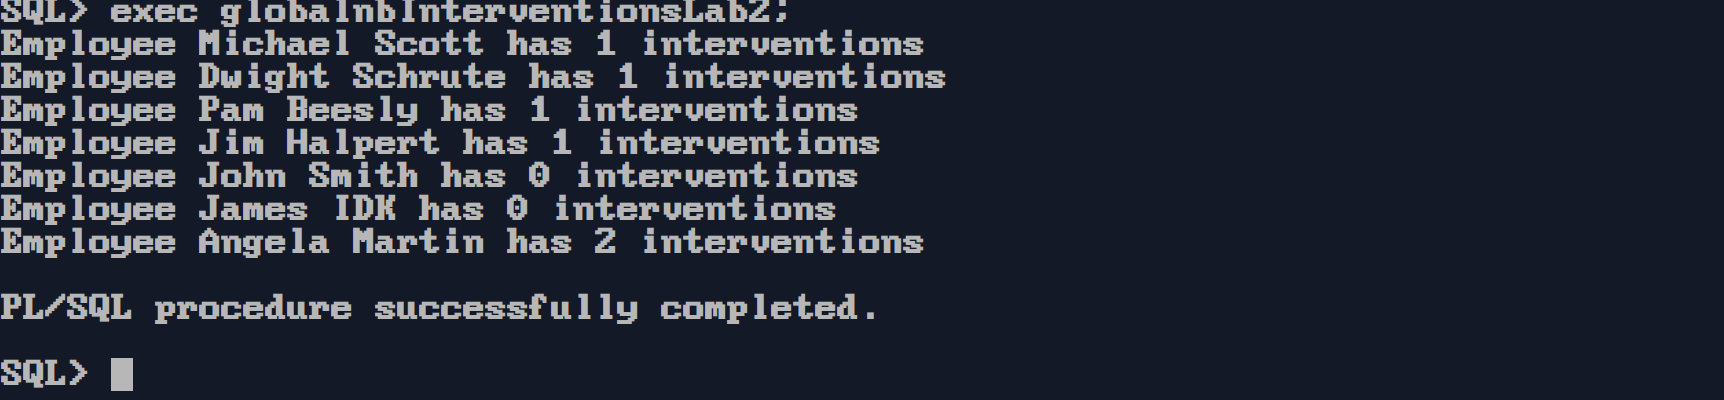
\includegraphics[width=\textwidth]{SQL/examples/PLSQL/EX1/PNG/ex6.png}
\end{figure}

\vspace{0.5cm}

\subsection*{7 Notify Model Was Added}

\lstinputlisting{SQL/examples/PLSQL/EX1/ex8.sql}

\vspace{0.25cm}
\begin{figure}[ht]
    \centering
    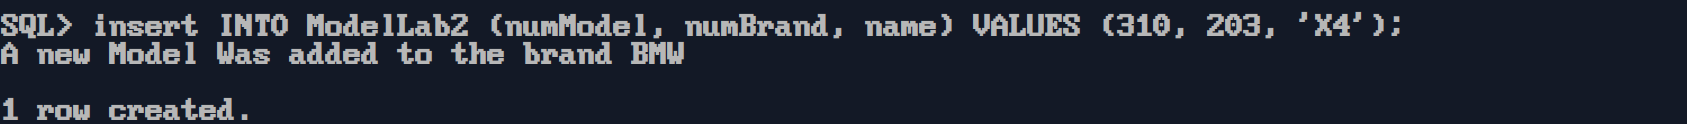
\includegraphics[width=\textwidth]{SQL/examples/PLSQL/EX1/PNG/ex8.png}
\end{figure}

\vspace{0.5cm}
\newpage
\subsection*{8 Check New Salary Before Updating}

\lstinputlisting{SQL/examples/PLSQL/EX1/ex9.sql}

\vspace{0.25cm}
\begin{figure}[ht]
    \centering
    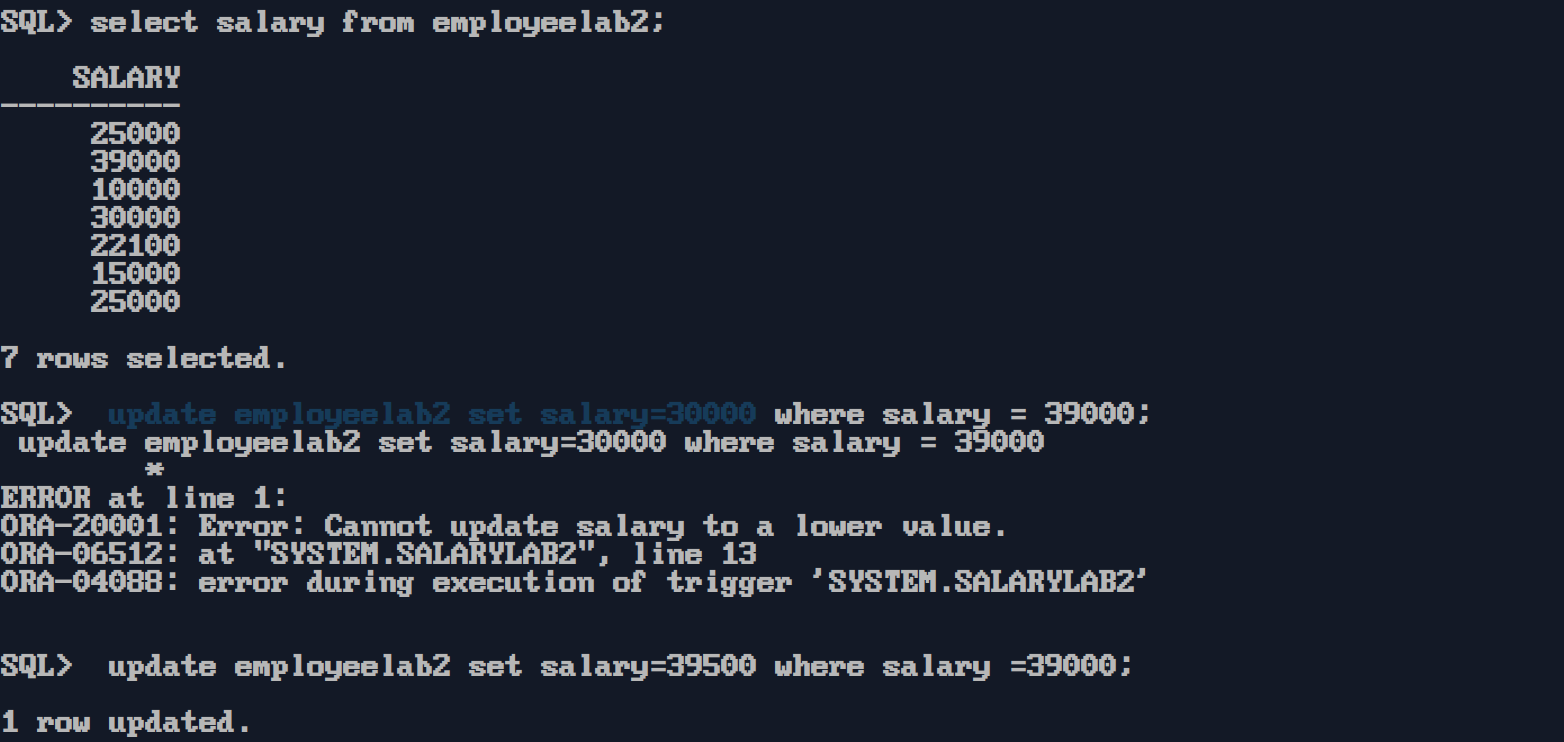
\includegraphics[width=\textwidth]{SQL/examples/PLSQL/EX1/PNG/ex9.png}
\end{figure}

\newpage
\subsection*{9 Check Period}

\lstinputlisting{SQL/examples/PLSQL/EX1/ex10.sql}

\subsection*{10 Add nb\_inter}

\lstinputlisting{SQL/examples/PLSQL/EX1/ex11.1.sql}

\vspace{0.25cm}
\begin{figure}[ht]
    \centering
    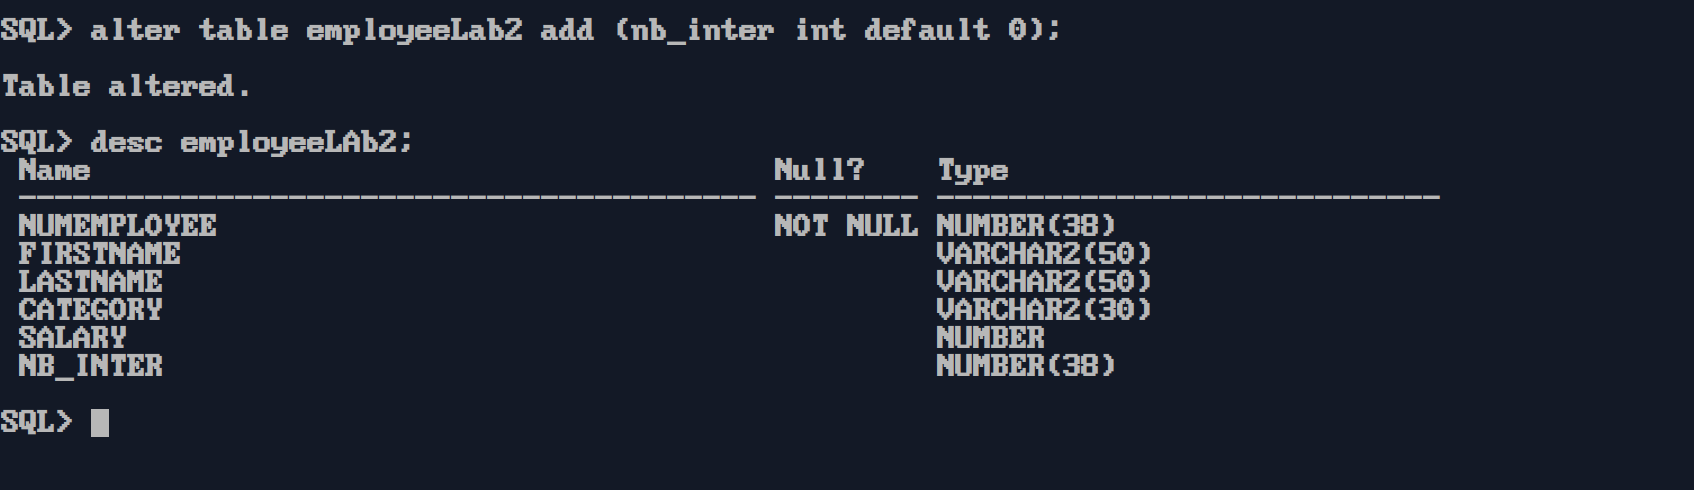
\includegraphics[width=\textwidth]{SQL/examples/PLSQL/EX1/PNG/ex11.1.png}
\end{figure}


\subsection*{11 Fill nb\_inter Procedure}

\lstinputlisting{SQL/examples/PLSQL/EX1/ex11.2.sql}

\vspace{0.25cm}
\begin{figure}[ht]
    \centering
    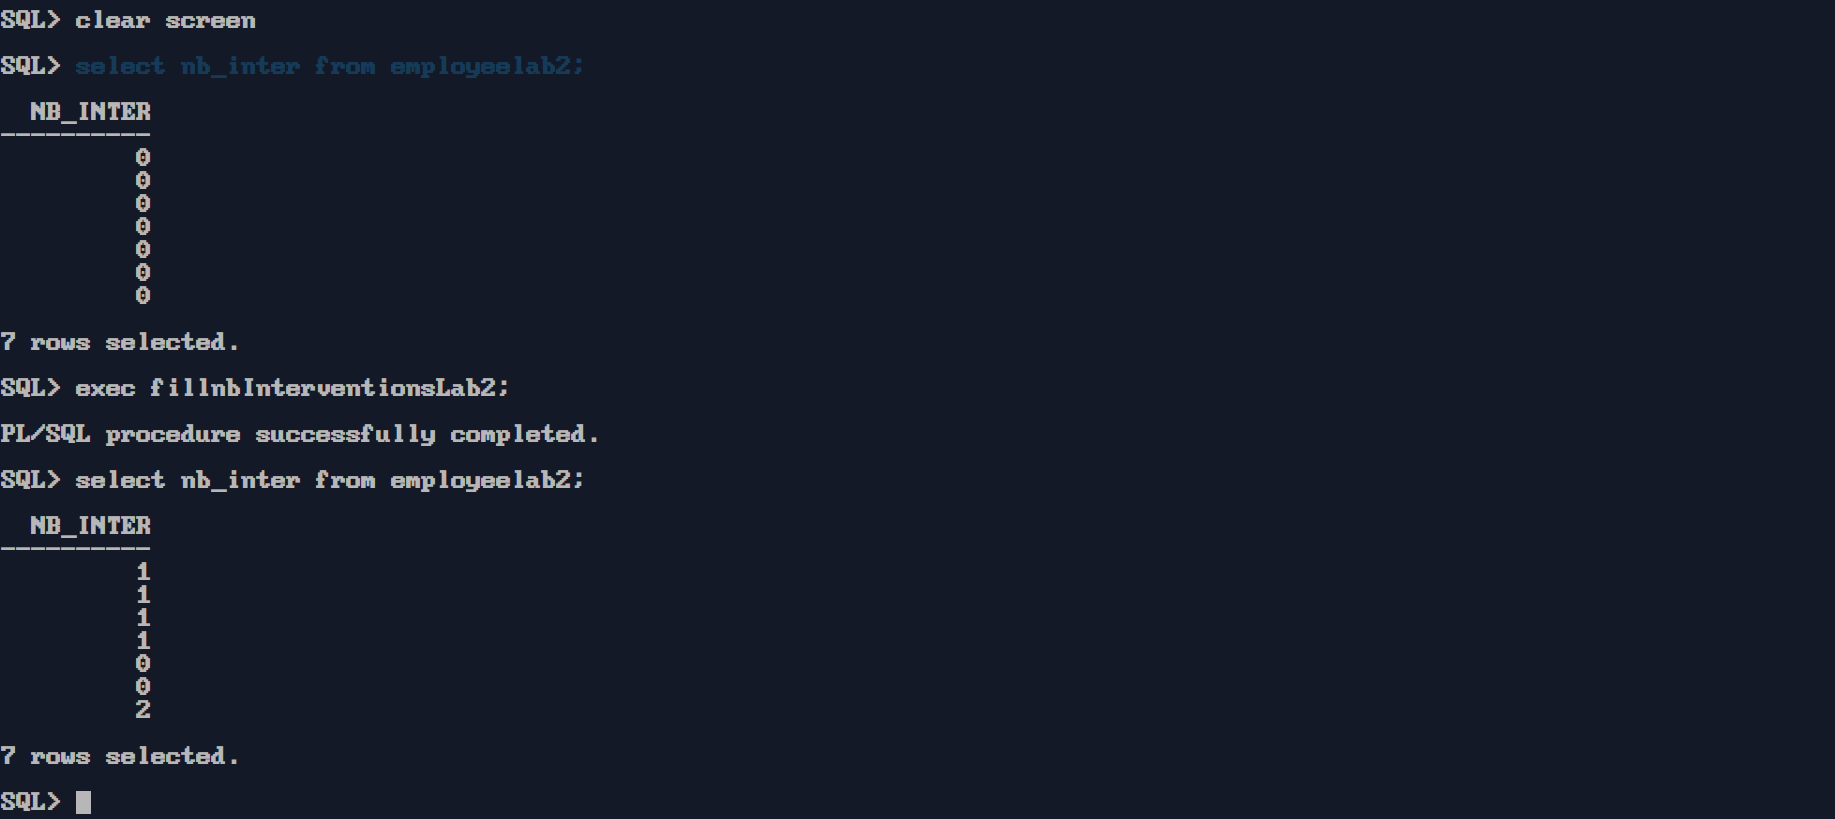
\includegraphics[width=\textwidth]{SQL/examples/PLSQL/EX1/PNG/ex11.2.png}
\end{figure}


\subsection*{12 }
\subsection*{12.1 Trigger After Insert}

\lstinputlisting{SQL/examples/PLSQL/EX1/ex11.3.1.sql}

\subsection*{12.2 Trigger After Delete}

\lstinputlisting{SQL/examples/PLSQL/EX1/ex11.3.2.sql}



\newpage
\begin{figure}[ht]
    \centering
    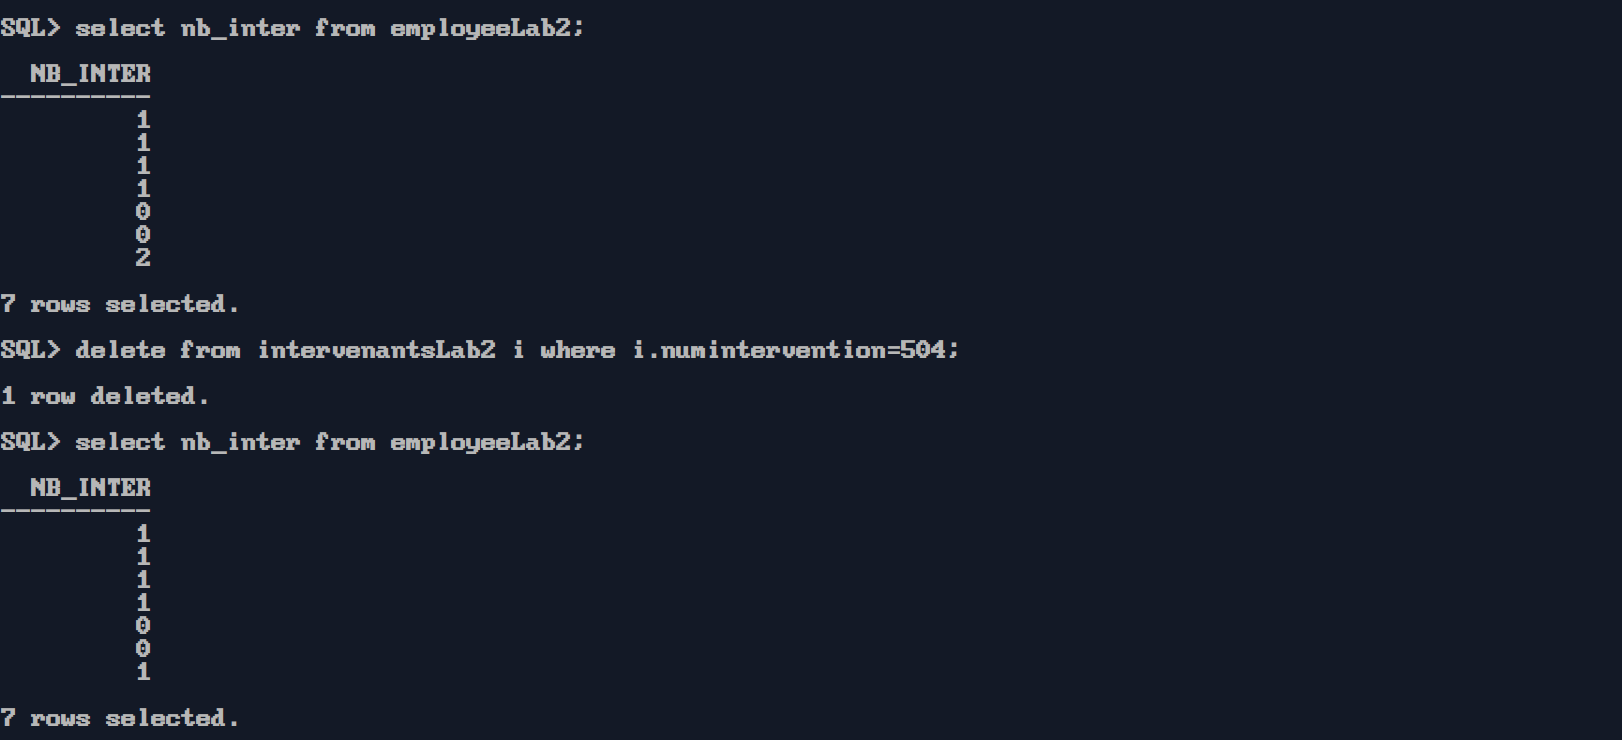
\includegraphics[width=\textwidth]{SQL/examples/PLSQL/EX1/PNG/ex11.3.png}
\end{figure}

\vspace{0.5cm}

\begin{prettyBox}{Note}{red}
Insert .sql code are inside the SQL/examples/PLSQL/EX1/insert folder
\end{prettyBox}

